\documentclass[twoside]{book}

% Packages required by doxygen
\usepackage{fixltx2e}
\usepackage{calc}
\usepackage{doxygen}
\usepackage[export]{adjustbox} % also loads graphicx
\usepackage{graphicx}
\usepackage[utf8]{inputenc}
\usepackage{makeidx}
\usepackage{multicol}
\usepackage{multirow}
\PassOptionsToPackage{warn}{textcomp}
\usepackage{textcomp}
\usepackage[nointegrals]{wasysym}
\usepackage[table]{xcolor}

% Font selection
\usepackage[T1]{fontenc}
\usepackage[scaled=.90]{helvet}
\usepackage{courier}
\usepackage{amssymb}
\usepackage{sectsty}
\renewcommand{\familydefault}{\sfdefault}
\allsectionsfont{%
  \fontseries{bc}\selectfont%
  \color{darkgray}%
}
\renewcommand{\DoxyLabelFont}{%
  \fontseries{bc}\selectfont%
  \color{darkgray}%
}
\newcommand{\+}{\discretionary{\mbox{\scriptsize$\hookleftarrow$}}{}{}}

% Page & text layout
\usepackage{geometry}
\geometry{%
  a4paper,%
  top=2.5cm,%
  bottom=2.5cm,%
  left=2.5cm,%
  right=2.5cm%
}
\tolerance=750
\hfuzz=15pt
\hbadness=750
\setlength{\emergencystretch}{15pt}
\setlength{\parindent}{0cm}
\setlength{\parskip}{3ex plus 2ex minus 2ex}
\makeatletter
\renewcommand{\paragraph}{%
  \@startsection{paragraph}{4}{0ex}{-1.0ex}{1.0ex}{%
    \normalfont\normalsize\bfseries\SS@parafont%
  }%
}
\renewcommand{\subparagraph}{%
  \@startsection{subparagraph}{5}{0ex}{-1.0ex}{1.0ex}{%
    \normalfont\normalsize\bfseries\SS@subparafont%
  }%
}
\makeatother

% Headers & footers
\usepackage{fancyhdr}
\pagestyle{fancyplain}
\fancyhead[LE]{\fancyplain{}{\bfseries\thepage}}
\fancyhead[CE]{\fancyplain{}{}}
\fancyhead[RE]{\fancyplain{}{\bfseries\leftmark}}
\fancyhead[LO]{\fancyplain{}{\bfseries\rightmark}}
\fancyhead[CO]{\fancyplain{}{}}
\fancyhead[RO]{\fancyplain{}{\bfseries\thepage}}
\fancyfoot[LE]{\fancyplain{}{}}
\fancyfoot[CE]{\fancyplain{}{}}
\fancyfoot[RE]{\fancyplain{}{\bfseries\scriptsize Generated by Doxygen }}
\fancyfoot[LO]{\fancyplain{}{\bfseries\scriptsize Generated by Doxygen }}
\fancyfoot[CO]{\fancyplain{}{}}
\fancyfoot[RO]{\fancyplain{}{}}
\renewcommand{\footrulewidth}{0.4pt}
\renewcommand{\chaptermark}[1]{%
  \markboth{#1}{}%
}
\renewcommand{\sectionmark}[1]{%
  \markright{\thesection\ #1}%
}

% Indices & bibliography
\usepackage{natbib}
\usepackage[titles]{tocloft}
\setcounter{tocdepth}{3}
\setcounter{secnumdepth}{5}
\makeindex

% Hyperlinks (required, but should be loaded last)
\usepackage{ifpdf}
\ifpdf
  \usepackage[pdftex,pagebackref=true]{hyperref}
\else
  \usepackage[ps2pdf,pagebackref=true]{hyperref}
\fi
\hypersetup{%
  colorlinks=true,%
  linkcolor=blue,%
  citecolor=blue,%
  unicode%
}

% Custom commands
\newcommand{\clearemptydoublepage}{%
  \newpage{\pagestyle{empty}\cleardoublepage}%
}

\usepackage{caption}
\captionsetup{labelsep=space,justification=centering,font={bf},singlelinecheck=off,skip=4pt,position=top}

%===== C O N T E N T S =====

\begin{document}

% Titlepage & ToC
\hypersetup{pageanchor=false,
             bookmarksnumbered=true,
             pdfencoding=unicode
            }
\pagenumbering{roman}
\begin{titlepage}
\vspace*{7cm}
\begin{center}%
{\Large P\+A02 }\\
\vspace*{1cm}
{\large Generated by Doxygen 1.8.11}\\
\end{center}
\end{titlepage}
\clearemptydoublepage
\tableofcontents
\clearemptydoublepage
\pagenumbering{arabic}
\hypersetup{pageanchor=true}

%--- Begin generated contents ---
\chapter{File Index}
\section{File List}
Here is a list of all documented files with brief descriptions\+:\begin{DoxyCompactList}
\item\contentsline{section}{\hyperlink{PA02_8cpp}{P\+A02.\+cpp} \\*Implements the program entry point }{\pageref{PA02_8cpp}}{}
\end{DoxyCompactList}

\chapter{File Documentation}
\hypertarget{PA02_8cpp}{}\section{P\+A02.\+cpp File Reference}
\label{PA02_8cpp}\index{P\+A02.\+cpp@{P\+A02.\+cpp}}


Implements the program entry point.  


{\ttfamily \#include $<$iostream$>$}\\*
{\ttfamily \#include $<$fstream$>$}\\*
{\ttfamily \#include $<$cstring$>$}\\*
{\ttfamily \#include $<$string$>$}\\*
Include dependency graph for P\+A02.\+cpp\+:\nopagebreak
\begin{figure}[H]
\begin{center}
\leavevmode
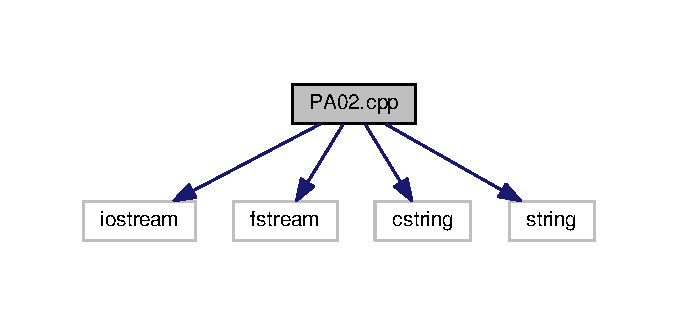
\includegraphics[width=326pt]{PA02_8cpp__incl}
\end{center}
\end{figure}
\subsection*{Functions}
\begin{DoxyCompactItemize}
\item 
int \hyperlink{PA02_8cpp_a38289856e74672ec95ce0fbb0ff279d5}{k\+Small} (int k\+Val, int $\ast$array, int first, int last, std\+::string \&log)
\begin{DoxyCompactList}\small\item\em Returns the kth smallest value in an arrray. \end{DoxyCompactList}\item 
int \hyperlink{PA02_8cpp_a3c04138a5bfe5d72780bb7e82a18e627}{main} (int argc, char $\ast$$\ast$argv)\hypertarget{PA02_8cpp_a3c04138a5bfe5d72780bb7e82a18e627}{}\label{PA02_8cpp_a3c04138a5bfe5d72780bb7e82a18e627}

\begin{DoxyCompactList}\small\item\em Entry point/main function of the program. \end{DoxyCompactList}\end{DoxyCompactItemize}


\subsection{Detailed Description}
Implements the program entry point. 

\begin{DoxyAuthor}{Author}
Matthew Bauer  File skeleton created by Shehryar Khattak for C\+S302 Spring 2016. 
\end{DoxyAuthor}


\subsection{Function Documentation}
\index{P\+A02.\+cpp@{P\+A02.\+cpp}!k\+Small@{k\+Small}}
\index{k\+Small@{k\+Small}!P\+A02.\+cpp@{P\+A02.\+cpp}}
\subsubsection[{\texorpdfstring{k\+Small(int k\+Val, int $\ast$array, int first, int last, std\+::string \&log)}{kSmall(int kVal, int *array, int first, int last, std::string &log)}}]{\setlength{\rightskip}{0pt plus 5cm}int k\+Small (
\begin{DoxyParamCaption}
\item[{int}]{k\+Val, }
\item[{int $\ast$}]{array, }
\item[{int}]{first, }
\item[{int}]{last, }
\item[{std\+::string \&}]{log}
\end{DoxyParamCaption}
)}\hypertarget{PA02_8cpp_a38289856e74672ec95ce0fbb0ff279d5}{}\label{PA02_8cpp_a38289856e74672ec95ce0fbb0ff279d5}


Returns the kth smallest value in an arrray. 


\begin{DoxyParams}{Parameters}
{\em k\+Val} & The value of k. \\
\hline
{\em array} & The array to search. W\+A\+R\+N\+I\+NG\+: is edited by the function. \\
\hline
{\em first} & The first item in the section of the array to search. \\
\hline
{\em last} & The last item in the section of the array to search. \\
\hline
{\em log} & The string to write the algorithm log into. \\
\hline
\end{DoxyParams}
\begin{DoxyPrecond}{Precondition}
last-\/first+1 $>$= k\+\_\+val 

log == \char`\"{}\char`\"{} 
\end{DoxyPrecond}
\begin{DoxyPostcond}{Postcondition}
The log parameter will be filled with a log report. 
\end{DoxyPostcond}
\begin{DoxyReturn}{Returns}
The kth smallest value in the given array. 
\end{DoxyReturn}

%--- End generated contents ---

% Index
\backmatter
\newpage
\phantomsection
\clearemptydoublepage
\addcontentsline{toc}{chapter}{Index}
\printindex

\end{document}
